\documentclass[conference]{IEEEtran}
\IEEEoverridecommandlockouts
\usepackage{graphicx}
\usepackage{paralist}
\usepackage{algorithm}
\usepackage{algorithmicx}
\usepackage{algpseudocode}
\usepackage[dvipsnames]{xcolor}
\usepackage{amsmath}
\usepackage{hyperref}
\usepackage{caption}
\usepackage{subcaption}
\usepackage{ulem}
\usepackage{xspace}
\usepackage{tabularx}
\usepackage{booktabs}
\usepackage{multirow}

% Fix link colors
\hypersetup{
    colorlinks = true,
    linkcolor=red,
    citecolor=red,
    urlcolor=blue,
    linktocpage % so that page numbers are clickable in toc
}

\algblock{Input}{EndInput}
\algnotext{EndInput}
\algblock{Output}{EndOutput}
\algnotext{EndOutput}
\newcommand{\Desc}[2]{\State \makebox[2em][l]{#1}#2}

\newcommand{\tristan}[1]{\color{orange}\textbf{From Tristan:}#1\color{black}}
\newcommand{\henri}[1]{\color{green}\textbf{From Henri:}#1\color{black}}
\newcommand{\english}[1]{\uwave{#1}}

\newcommand{\simgrid}{SimGrid\xspace}
\newcommand{\wrench}{WRENCH\xspace}

\newcommand{\valerie}[1]{\color{blue}\textbf{From Valerie:}#1\color{black}}


\begin{document}

\title{Modeling the Linux page cache for accurate simulation of data-intensive applications}

\author{
  \IEEEauthorblockN{
    Hoang-Dung Do\IEEEauthorrefmark{1},
    Val\'erie Hayot-Sasson\IEEEauthorrefmark{1},
    Rafael Ferreira da Silva\IEEEauthorrefmark{3},
    Christopher Steele\IEEEauthorrefmark{4},
    Henri Casanova\IEEEauthorrefmark{2},
    Tristan Glatard\IEEEauthorrefmark{1}
  }\\
  \IEEEauthorblockA{
    \IEEEauthorrefmark{1}Department of Computer Science and Software Engineering, Concordia University, Montreal, Canada\\
    \IEEEauthorrefmark{2}Department of Information and Computer Sciences, University of Hawai`i at M\=anoa, USA\\
    \IEEEauthorrefmark{3}Information Sciences Institute, University of Southern California, Marina Del Rey, CA, USA\\
    \IEEEauthorrefmark{4}Department of Psychology, Concordia University, Montreal, Canada
  }
}

\maketitle

    \begin{abstract}

    % Henri Rewrote quite  a bit in the next paragraph here to spell out a bit
    % more why we need simulation
    The emergence of Big Data in recent years has resulted in a growing
    need for efficient data storage management techniques.  While
    infrastructures with sufficient compute power are available to
    process large datasets, the I/O bottleneck remains.  A
    well-known approach for reducing the overhead of
    I/O operations is to use the Linux page cache.  It is thus crucial
    to study experimentally the impact of the Linux page cache on the
    performance of Big Data applications. Given the difficulties with and shortcomings of
    real-world experiments, a popular approach for application
    performance studies is to use simulation.  While many simulation
    frameworks have been developed for this purpose, they do not 
    simulate page caching fully, or even at all.  As a result, using
    these frameworks for studying the performance of data-intensive
    applications leads to inaccurate simulation results. 

    In this paper, we propose a I/O simulation model that characterizes
    the key features of the page cache. We have implemented this model
    as  part of the \wrench workflow simulation framework, which itself
    builds on the popular \simgrid distributed systems simulation
    framework.  Our model and its implementation enable the simulation
    of both single-threaded and multithreaded applications, and of both
    writeback and writethrough caches for local or network-based
    filesystems. We evaluate the accuracy of our model in different
    conditions, including sequential and concurrent applications, as
    well as local and remote I/Os.  We find that our page cache model
    reduces the simulation error by up to an order of magnitude when
    compared to state-of-the-art, cacheless simulations.

    \end{abstract}

    \section{Introduction}

        The Linux Page Cache plays an important role in
        reducing filesystem data transfer times. With the page cache, previously
        read data can be re-read directly from memory and written data can be written to
        memory before being asynchronously flushed to disk, resulting in improved I/O performance
        on slower storage devices. The performance improvements
        depend on many factors including the total amount of memory,
        the amount of data being written (i.e., dirty data), and the amount of memory available for
        written data. All these factors are important when determining the impact of I/O on
        application performance, particularly in data-intensive applications.

        % Swapped the order the two paragraphs and merged them into one
        The number of data-intensive applications has been steadily rising as a result of
        open-data and data sharing initiatives. Due to the sheer size of the data being
        processed, these applications must be executed on large-scale infrastructures
    such as High Performance Computing (HPC) clusters or the cloud.  It
    is thus crucial to quantify the performance of these applications
    on these platforms. The goals include determining which type of hardware/software
    stacks are best suited to different application classes, as well as
    understanding the shortcomings of current algorithms, designs and
    technologies so as to propose new solutions. Unfortunately, application performance
        studies via experiments on real-world compute platforms
        face several difficulties (high operational costs, labor-intensive experimental setups,
        shared platforms with dynamic loads that hinder reproducibility of results) and shortcomings
        (experiments are limited to the available platform/software configurations, which precludes
        the exploration of hypothetical scenarios). 
    Simulations address these concerns by providing models
    and abstractions for the performance of computer hardware, such as
    CPU, network and storage. As a result, simulations provide a
    cost-effective, fast, easy and reproducible way to evaluate
    application performance on arbitrary platform configurations. It thus comes
        as no surprise that, considering here only the field of parallel and distributed
        computing, a large number of simulation frameworks have been developed and used
        to support research and development endeavors~\cite{ optorsim, gridsim, groudsim, cloudsim, nunez2012simcan,nunez2012icancloud, mdcsim, dissect_cf, cloudnetsimplusplus, fognetsimplusplus, casanova2014simgrid, ROSS, casanova2020fgcs}. 


        Page caching is an ubiquitous technique for mitigating the I/O bottleneck
        faced by data-intensive applications. As such, it is necessary to simulate page caching
        when performing performance studies in simulation.
        Furthermore, simulating the page cache makes it possible to study relevant application-I/O
        bottlenecks that can arise over the course of execution, such as page cache
        starvation~\cite{zhuang2017}.
        While existing simulation frameworks of parallel and distributed computing
        systems  capture many relevant features of hardware/software stacks, 
        they lack the ability to simulate page cache adequately. Those frameworks
        that implement some page cache simulation
        fail to capture key features such
        as dirty data and cache eviction policies~\cite{nunez2012simcan,nunez2012icancloud}. 
        Some simulators, such as that in~\cite{xu2018saving}, do capture such features
        but are domain-specific. 

        %However, there is a trade-off between accuracy and scalability, which has been
        %indicated in some reviews \cite{casanova2014simgrid} \cite{byrne2017review}.
        %This means that in most cicumstances, users have to, more or less, sacrifice
        %accuracy for the scalability and performance when their platforms grow to
        %hundreds or thousands nodes.

    In this work, we present \wrench-cache, a simulation model of I/O
    with page cache incorporated into the \wrench simulation framework~\cite{casanova2020fgcs},
    which is  based on the popular \simgrid distributed simulation framework~\cite{casanova2014simgrid}.
    The added value of \wrench-cache is to make it possible to simulate 
        application execution accurately in the presence of page caching. Our specific 
        contributions are as follows:
    \begin{compactitem}
        \item A page cache simulation model that supports 
    both single-threaded and multithreaded applications, and of both
    writeback and writethrough caches for local or network-based
    filesystems;
        \item An implementation of this model in \wrench; 
        \item An evaluation of the accuracy and scalability of our model, and of its implementation,
              for a range of applications, platforms, and page cache configurations. 
    \end{compactitem}


    \section{Related Work}
    \label{relatedwork}

        \subsection{Page cache}

        To improve performance of disk accesses, the page cache was introduced to the Linux kernel. %It contains pages referring to physical pages on disk \cite{linuxdev3rd2010}.
        The goal of the page cache is to ensure that most I/O operations occur entirely
        within memory space rather than synchronously to and from storage devices.
        All disk-backed data located in the page cache are partitioned into many small pages.
        When a read operation is initiated, the kernel checks whether the required pages are in memory.
        If it is the case, data is read entirely from memory (i.e. \textit{cache hit}). Otherwise,
        the necessary pages must be loaded to memory from the disk (i.e. \textit{cache miss}).
        Conversely, for writing, one of three strategies can be applied: direct~I/O (or, ``no-write''),
        writethrough and writeback.
        If direct~I/O is enabled for a given file system, all I/O operations bypass the
        page cache for writes, writing data directly to disk. In contrast, writethrough enables the page cache
        for file system writes, but the data is written synchronously from memory to disk. Writeback extends writethrough
        by enabling asynchronous writes to disk, meaning that a write call will return once
        the data has been written to memory.
        The writeback strategy is considered to outperform writethrough as well as
        direct I/O as it delays disk writes to perform a bulk write at a later time
        \cite{linuxdev3rd2010}.
        Cache eviction and flushing strategies are integral to proper page cache functioning.
        Whenever space in memory becomes limited, either as a result of application memory
        or page cache use, page cache data may be evicted. Only data that
        has been persisted to storage (clean pages) can be flagged for eviction and removed from
        memory. Written data that has not yet been persisted to disk (dirty data) must first
        be copied (flushed) to storage prior to eviction. When sufficient memory is
        being occupied, the flushing process is synchronous. However, even when
        there is sufficient available memory, written data will be flushed to disk
        at a predefined interval through a process known as \textit{periodical flushing}.
        Periodical flushing only flushes expired dirty pages, which remain dirty in
        page cache longer than an expiration time configured in the kernel.
        Different cache eviction algorithms have also been developed and proposed
        \cite{owda2014comparison}.
        The Linux kernel uses a two-list strategy to flag pages for eviction.
        The two-list strategy is based on a least recently used (LRU) policy
        and uses an active and inactive list in its implementation.
        If accessed pages are not in the page cache, they are added to the inactive list.
        Should pages located on the inactive list be accessed, they will be moved from
        the inactive to the active list.
        The lists are also kept balanced by moving pages from the active list
        to the inactive list when the active list grows too large.
        Thus, the active list only contains pages which are accessed more than once
        and not evictable, while the inactive list includes pages accessed once only,
        or pages that have be accessed more than once but moved from the active list.
        Both lists operate using LRU eviction policies meaning the data that has
        not be accessed recently will be moved first.

        \subsection{Simulation}

        Many simulation frameworks have been developed to enable the
        simulation of parallel and distributed
        applications~\cite{optorsim, gridsim, groudsim, cloudsim,
        nunez2012simcan,nunez2012icancloud, mdcsim, dissect_cf,
        cloudnetsimplusplus, fognetsimplusplus, casanova2014simgrid,
        ROSS, casanova2020fgcs}. These frameworks implement simulation
        models and abstractions to aid the development of simulators
        for studying the functional and performance behaviors of
        application workloads executed on various hardware/software
        infrastructures. 

        The two main concerns for simulation are \emph{accuracy}
        (the ability to faithfully reproduce real-world executions) and
        \emph{scalability}  (the ability to simulate large/long real-world
        executions quickly and with low RAM footprint). The above
        frameworks achieve different compromises between the two.  At
        one extreme are discrete-event models that capture
        ``microscopic'' behaviors of hardware/software systems (e.g.,
        packet-level network simulation, block-level disk simulation,
        cycle-accurate CPU simulation), which favor accuracy over
        speed.  At the other extreme are analytical models that capture
        ``macroscopic'' behaviors via mathematical models.  While these
        models lead to fast simulation, they must be developed
        carefully if high levels of accuracy are to be
        achieved~\cite{velhoTOMACS2013}. 

        In this  work, we use the \simgrid and \wrench simulation
        frameworks.  The years of research and development invested in
        the popular \simgrid simulation framework~\cite{casanova2014simgrid}, have
        culminated in a set of state-of-the-art macroscopic simulation
        models that yield high accuracy, as demonstrated by
        (in)validation studies and comparisons to competing
        frameworks~\cite{smpi_validity, velhoTOMACS2013, simutool_09,
        nstools_07, lebre2015, pouilloux:hal-01197274,
        smpi_tpds2017,  7885814, 8048921, 7384330}.  But one
        significant drawback of \simgrid is that its simulation
        abstractions are low-level, meaning that implementing a
        simulator of complex systems can be
        labor-intensive~\cite{kecskemeti_2014}. To remedy this problem,
        the \wrench simulation framework~\cite{casanova2020fgcs}
        builds on top of \simgrid to provide higher-level simulation
        abstractions, so that simulators of complex applications and
        systems can be implemented with a few hundred lines.

        Although the Linux page cache has a large impact on I/O
        performance, and thus on the execution of data-intensive
        applications, its simulation is rarely considered in the above
        frameworks.  Most frameworks merely simulate I/O operations
        based on storage bandwidths and capacities.  The SIMCAN
        framework does models page caching by storing data accessed on
        disk in a block cache~\cite{nunez2012simcan}.  Page cache is
        also modeled in iCanCloud through a component that manages
        memory accesses and cached data~\cite{nunez2012icancloud}.
        However, the scalability of the iCanCloud simulator is limited
        due to it using  microscopic simulation models.  Besides, none
        of these simulators provide any writeback cache simulator nor
        cache eviction policies through LRU lists.  Although cache
        replacement policies are applied in~\cite{xu2018saving} to
        simulate in-memory caching, their simulator is specific to
        energy consumption of multi-tier heterogeneous networks.

        In this study, we develop a page cache simulation model which we implement
        as part of the \wrench framework. We targeted \wrench because it is a
        recent, actively developed framework that provides convenient simulation
        abstractions, because it is easy to incorporate new simulation models
        into it, and because it builds on \simgrid, whose scalable and accurate
        simulation models we can thus reuse for our purpose. 

    \section{Methods}
    \label{method}
    We separate our simulation model in two components, the I/O
    Controller and the Memory Manager, which together simulate
    file reads and writes (Figure~\ref{fig:interaction}).
    To read or write a file chunk, a simulated application sends a
    request to the I/O Controller. The I/O Controller interacts as needed with
    the Memory Manager to free memory through flushing or eviction,
    and to read or write cached data. The Memory Manager
    implements these operations, simulates periodical flushing
    and eviction, and reads or writes to disk when necessary.
    In case the writethrough strategy is used, the I/O Controller directly writes to disk, 
    cache is flushed if needed and written data is added to page cache.

    \begin{figure}
           \centering
           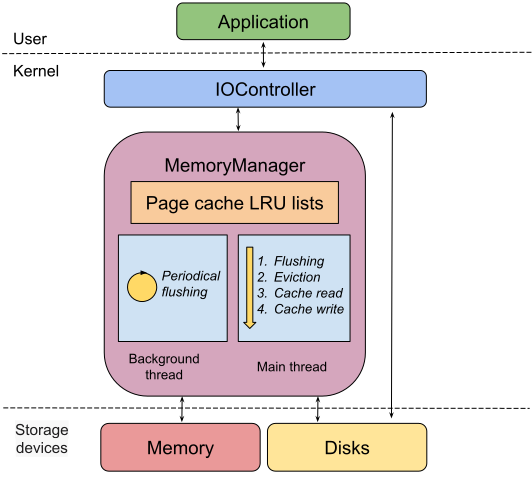
\includegraphics[width=0.85\columnwidth]{figures/interaction.pdf}
           \caption{Overview of the page cache simulator.
           Applications send file read or write requests to the
           I/O Controller that orchestrates flushing, eviction, cache
           and disk accesses with the Memory Manager. Concurrent accesses to storage
           devices (memory and disk) are simulated using existing models.}
           \label{fig:interaction}
    \end{figure}

    \subsection{Memory Manager}

    The Memory Manager simulates two parallel threads: the main one
    implements flushing, eviction, and cached I/Os synchronously, whereas
    the second one, which operates in the background, periodically searches for
    expired dirty data in page cache LRU lists and flushes this data to disk. We
    use existing storage simulation models~\cite{lebre2015} to simulate disk and
    memory, characterized by their storage capacity, read and write
    bandwidths, and latency. These models account for
    bandwidth sharing between concurrent memory accesses and concurrent disk accesses.

    \subsubsection{Page cache LRU lists}

    In the Linux kernel, page cache LRU lists contain file pages. However,
    due to the large number of file pages, simulating lists of pages
    induces substantial overhead.
    Therefore, we introduce the concept of a data block as a unit to represent data
    cached in memory. A data block is a subset of file pages stored in
    page cache that were accessed in the same I/O operation.
    A data block has information about the file name, block size, last access
    time, a dirty flag that represents whether the data is clean (0)
    or dirty (1), and an entry (creation) time.
    Blocks can have different sizes and a given file can have multiple
    data blocks in page cache. In addition, a data block can be split into an
    arbitrary number of smaller blocks.
    \begin{figure}
           \centering
           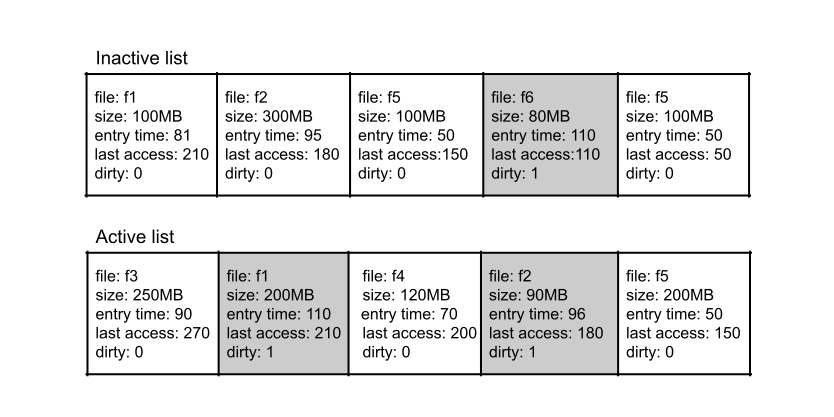
\includegraphics[width=\columnwidth]{figures/lru_lists.pdf}
           \caption{Model of page cache LRU lists with data blocks.}
           \label{fig:lrulist}
    \end{figure}

    We model page cache LRU lists as
    two lists of data blocks, an active list and an inactive list, both ordered by
    last access time (earliest first, see Figure~\ref{fig:lrulist}).
    As in the kernel, our simulator limits the size of the active list to
    twice the size of the inactive list, by moving least recently
    used data blocks from the active list to the inactive list~\cite{gorman2004understanding, linuxdev3rd2010}.

    At any given time, a file can be partially cached, completely cached,
    or not cached at all. A cached data block can only reside in one of two
    LRU lists. The first time they are accessed, blocks are
    added to the inactive list. On subsequent accesses, blocks of the
    inactive list are moved to the top of the active list. Cached blocks
    written to cache are marked as dirty until they are flushed to disk.

    \subsubsection{Reads and writes}

    Our simulation model supports chunk-by-chunk file accesses
    with a user-defined chunk size. However, for simplicity, we assume that file pages are
    accessed in a round-robin fashion rather than fully randomly.
    Therefore, when a file is read, cached data is read only after all uncached data was read, and data from the inactive list is read
    before data from the active list
    (data reads occur from left to right in Figure~\ref{fig:read_order}).
    When a chunk of \emph{uncached} data is read, a new clean block is created
    and appended to the inactive list.
    When a chunk of \emph{cached} data is read, one or more existing data blocks in the LRU lists are accessed.
    If these blocks are clean, we merge them together, update the access time and size of the resulting block,
    and append it to the active list.
    If the blocks are dirty, we move them independently to the active list, to preserve their entry time.
    Because the chunk and block sizes may be different, there are situations
    where a block is not entirely read.
    In this case, the block is split in two smaller blocks and one of them is re-accessed.
    % From Tristan: not sure where to put this nor if it's necessary:
    % , in which chunks are read/written
    % until file is entirely read/written.
    \begin{figure}
           \centering
           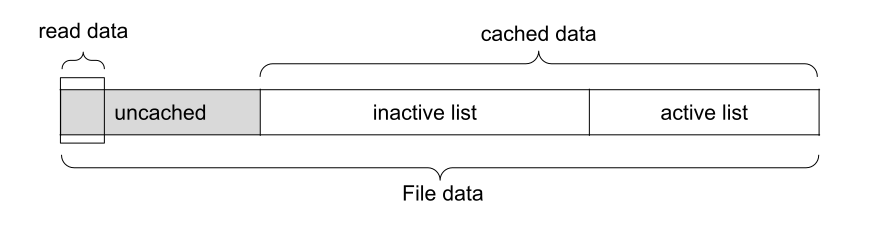
\includegraphics[width=\columnwidth]{figures/read_order.pdf}
           \caption{File data read order. Data is read from left to right: uncached data
           is read first, followed by data from the inactive list, and finally data from the active list. }
           \label{fig:read_order}
    \end{figure}

    For file writes, we assume that all data to be written is
    uncached. Thus, each time a chunk is written, we create a block of dirty data
    and append it to the inactive list.

    \subsubsection{Flushing and eviction}

    The main simulated thread in the Memory Manager can flush or evict data from the
    memory cache. The data flushing simulation
    function takes the amount of data to flush as parameter. While
    the amount of data to flush is not reached and there are dirty
    blocks remaining in cache, this function traverses the sorted
    inactive list, then the sorted active list, and writes the
    least recently used dirty block to disk, having set its dirty
    flag to 0. In case the amount of data to flush requires that a
    block be partially flushed, the block is split in two blocks,
    one that is flushed and one that remains dirty. The time needed
    to flush data to disk is simulated by the storage model.

    The cache eviction simulation also runs in
    the main thread. It frees up the page cache by traversing and deleting
    least recently used clean data blocks in the inactive list.
    The amount of data to evict is passed as a parameter and data blocks are deleted
    from the inactive list until the evicted data reaches the required amount,
    or until there is no clean block left in the list.
    If the last evicted block does not have to be entirely evicted, the block is split in two blocks,
    and only one of them is evicted.
    The overhead of the cache eviction algorithm is not part of the simulated time
    since cache eviction time is negligible in real systems \tristan{a reference would be welcome}.

    \begin{algorithm}\caption{Periodical flushing simulation in I/O Controller}\label{alg:pdflush}
        \small
        \begin{algorithmic}[1]
            \Input
                \Desc{in}{page cache inactive list}
                \Desc{ac}{page cache active list}
                \Desc{t}{predefined flushing time interval}
                \Desc{exp}{predefined expiration time}
                \Desc{sm}{storage simulation model}
               \EndInput
               \While{host is on}
                \State blocks = expired\_blocks(exp, in) + expired\_blocks(exp, ac)
                \State flushing\_time = 0
                \For{blk in blocks} 
                  \State blk.dirty = 0 
                  \State flushing\_time = flushing\_time + sm.write(blocks)
                \EndFor
                \If{flushing\_time $<$ t}
                    \State sleep(t - flushing\_time)
                \EndIf  
            \EndWhile
        \end{algorithmic}
    \end{algorithm}

    Periodical flushing is simulated in the Memory Manager
    background thread. As in the Linux kernel, a dirty block
    in our model is considered expired if
    the duration since its entry time is longer than a
    predefined expiration time.
    Periodical flushing is simulated as an infinite loop in which
    the Memory Manager searches for dirty blocks and flushes them to disk (Algorithm~\ref{alg:pdflush}).
    % From Tristan: the algorithm is quite straightforward, I don't think this is
    % necessary
    % In each repetition, Memory Manager finds expired dirty blocks in two
    % page cache LRU lists (line 8), simulates writes of data of these blocks
    % to disk (line 9), and mark them as clean (line 10).
    % If the flushing time does not exceed our time interval, the thread is put
    % to sleep for the remaining time (lines 11-13).
    % Then based on the state of the host at current simulated time,
    % the algorithm continues or finishes the loop.
    Because periodical flushing is simulated as a background thread, it can happen concurrently
    with disk I/O initiated by the main thread. This is taken into account by the
    storage model and reflected in simulated I/O time.

    \subsection{I/O Controller}

    \begin{algorithm}\caption{File chunk read simulation in the I/O Controller}
    \label{alg:read}
        \small
        \begin{algorithmic}[1]
            \Input
                \Desc{cs}{chunk size}
                \Desc{fn}{file name}
                \Desc{fs}{file size (assumed to fit in memory)}
                \Desc{mm}{MemoryManager object}
                \Desc{sm}{storage simulation model}
               \EndInput
               \State disk\_read = min(cs, fs - mm.cached(fn)) \Comment{To be read from disk}
               \State cache\_read = cs - disk\_read \Comment{To be read from cache}
               \State required\_mem = cs + disk\_read
               \State mm.flush(required\_mem - mm.free\_mem - mm.evictable, fn)
               \State mm.evict(required\_mem - mm.free\_mem, fn)
               \If {disk\_read $>$ 0}  \Comment{Read uncached data}
               \State sm.read(disk\_read)
               \State mm.add\_to\_cache(disk\_read, fn)
               \EndIf
               \If {cache\_read $>$ 0} \Comment{Read cached}
               \State mm.cache\_read(cache\_read)
            \EndIf
            \State mm.use\_anonymous\_mem(cs)
        \end{algorithmic}
    \end{algorithm}
    As mentioned previously, our model reads and writes file chunks in a
    round-robin fashion. To read a file chunk, simulated applications send
    chunk read requests to the I/O Controller which processes them using
    Algorithm~\ref{alg:read}. First, we calculate the amount of uncached
    data that needs to be read from disk, and the remaining amount is read
    from cache (line 7-8). The amount of memory required to read the chunk
    is calculated, corresponding to a copy of the chunk in anonymous memory
    and a copy of the chunk in cache (line 9).
    If there is not enough available memory, the Memory Manager is called
    to flush dirty data (line 10). If necessary, flushing is complemented by
    eviction (line 11). Note that, when called with negative arguments, functions
    \texttt{flush} and \texttt{evict} simply return and do not do anything. Then,
    if the block requires
    uncached data, the memory manager is called to read data from disk and to add this
    data to cache (line 14).
    If cached data needs to be read, the Memory Manager is called to simulate
    a cache read  and update the corresponding data blocks accordingly (line 17).
    Finally, the memory manager is called to reduce the amount of free memory
    corresponding to the amount of anonymous memory used by application (line 19).

    \begin{algorithm}\caption{File chunk write simulation in the I/O Controller}
    \label{alg:write}
        \small
        \begin{algorithmic}[1]
            \Input
                \Desc{cs}{chunk size}
                \Desc{fn}{file name}
                \Desc{mm}{MemoryManager object}
               \EndInput
            \State remain\_dirty = dirty\_ratio * mm.avail\_mem - mm.dirty
            \If {remain\_dirty $>$ 0} \Comment{Write to memory}
                \State mm.evict(min(cs, remain\_dirty) - mm.free\_mem)
                \State mem\_amt = min(cs, mm.free\_mem)
                \State mm.write\_to\_cache(fn, mem\_amt)
            \EndIf
            \State remaining = cs - mem\_amt
            \While {remaining $>$ 0}  \Comment{Flush to disk, then write to cache}
                \State mm.flush(cs - mem\_amt)
                \State mm.evict(cs - mem\_amt  - mm.free\_mem)
                \State to\_cache = min(remaining, mm.free\_mem)
                \State mm.write\_to\_cache(fn, to\_cache)
                \State remaining = remaining - to\_cache
            \EndWhile

        \end{algorithmic}
    \end{algorithm}
    Algorithm~\ref{alg:write} describes our simulation of chunk writes in
    the I/O Controller.
    % Data is written to cache until the amount of dirty data in the cache
    % exceeds the dirty ratio times the amount of available memory. Data is then written to disk.
    Our algorithm initially checks the  amount of dirty data that
    can be written given the dirty ratio (line 5).
    If this amount is greater than 0, the Memory Manager is requested to evict
    data from cache if necessary (line 7).
    After eviction, the amount of data that can be written to
    page cache is calculated (line 8), and a cache write is simulated (line 9).
    If the dirty threshold is reached and there is remaining data to be written,
    the remaining data is written to cache in a loop
    where we repeatedly flush and evict to free space in the cache (line 12-18).

    The above models page cache in writeback
    mode. Our model also includes a write function in writethrough mode,
    which simply simulates a disk write with the amount of data passed in,
    then evicts cache if needed and adds the written data to the cache.

        \subsection{Implementation}

            We first created a standalone prototype
            simulator to evaluate the accuracy and correctness of our
            model in a simple scenario before integrating it in the more complex
            \wrench framework.
            The prototype uses the following basic storage model for
            both memory and disk:
            \begin{align*}
                & t_{r} = D / b_r \\
                & t_{w} = D / b_w\
            \end{align*}

            where:
            \begin{itemize}
                \item $t_{r}$ is the data read time
                \item $t_{w}$ is the data write time
                \item $D$ is the amount of data to read or write
                \item $b_r$ is the read bandwidth of the device
                \item $b_w$ is the write bandwidth of the device
            \end{itemize}

            This prototype does not simulate  bandwidth sharing and thus does not support
            concurrency: it is limited to single-threaded applications running on systems
            with a single-core CPU. We used this prototype for a first validation of our simulation
            model against a real sequential application running on a real system.
            The source code this prototype is available at
            \url{https://github.com/big-data-lab-team/paper-io-simulation/tree/master/exp/pysim}. We used Python 3.7.

            We also implemented our model as part of \wrench, enhancing its
            internal implementation and APIs with a page cache abstraction,
            and allowing users to activate the feature via a command-line
            argument. We used SimGrid's locking mechanism to handle
            concurrent accesses to page cache LRU lists by the two Memory
            Manager threads. For the experiments in this paper we use
            \wrench 1.6 at commit
            \href{https://github.com/wrench-project/wrench/tree/67185374330d2c4bf274fce222c937e838df5b03}{6718537433},
            which uses \simgrid 3.25, available at
            \url{https://framagit.org/simgrid/simgrid}. Our implementation
            is now part of \wrench's master branch and will be available to
            users with the upcoming \wrench 1.8 release. \wrench provides a full \simgrid-based simulation 
            environment that supports, among other features, concurrent accesses to storage devices, 
            applications distributed on multiple hosts, network transfers, 
            and multi-threading. 

        \subsection{Experiments}

        Our experiments compare real executions with our Python prototype,
        with the original \wrench, and with our \wrench-cache extension. We
        evaluate our page cache simulation in single-threaded and
        multi-threaded applications, accessing data on local and remote
        file systems. We use two applications: a synthetic one created to
        evaluate the simulation model, and a real one representative of
        neuroimaging data processing.

        The synthetic application, implemented in C, consists of three single-core,
        sequential tasks where each task reads the file produced by the
        previous task, increments every byte of this file to emulate real
        processing, and writes the resulting data to disk. Files are
        numbered by ascending creation times: File 1 is file read by Task 1, and File \texttt{i+1} is the file
        written by task \texttt{i}. In real executions, we clear the page
        cache before starting the application, to ensure comparable
        conditions among the runs. The anonymous memory used by application
        is released after each task, which we also simulate in the Python
        prototype and in WRENCH-cache.
        
        The real application is a workflow of the Nighres
        toolbox~\cite{huntenburg2018nighres} that implements skull
        stripping in high-resolution brain images, an operation common to
        many neuroimage analysis pipelines. The workflow is implemented as a Python
        script that calls Java image-processing routines. We used Python
        3.6, Java 8, and Nighres 1.3.0. We patched the
        skull stripping workflow to monitor task CPU times and inject them
        in the simulation, to focus our analysis on I/O times, the patched code is 
        available at \url{https://github.com/dohoangdzung/nighres}. 

        The applications were executed on a dedicated cluster at
        Concordia University, with one login node, 9 compute nodes, and 4
        storage nodes connected with a network bandwidth of 25 Gbps. Each
        compute node has 2 $\times$ 16-core Intel(R) Xeon(R) Gold 6130 CPU
        @ 2.10GHz, 250~GiB of RAM, 6 $\times$ SSDs of 450~GiB each with the XFS
        file system, 378~GiB of tmpfs, and 126~GiB of devtmpfs file system.
        Nodes run CentOS~8.1 with NFS version 4. We use the \texttt{atop}
        and \texttt{collectl} tools to monitor and collect memory status
        and disk throughput.

        To parametrize our simulators, we benchmarked the
        memory, local disk, remote disk (NFS), and network bandwidths
        (Table~\ref{table:benchmark}). Since \simgrid, and thus \wrench, currently only supports
        symmetrical bandwidths, we use the mean of the read and write
        bandwidth values in our experiments.
            \begin{table}
            \centering
            \begin{tabularx}{\columnwidth}{ll
            >{\centering\arraybackslash}X
            >{\centering\arraybackslash}X
            >{\centering\arraybackslash}X}
            \toprule
                \multicolumn{2}{c}{Bandwidths}  & Cluster (real) & Python prototype & \wrench simulator\\
            \midrule
            \multirow{2}{*}{Memory}      & read  & 6860 & 4812 & 4812\\
                                         & write & 2764 & 4812 & 4812\\
            \multirow{2}{*}{Local disk}  & read  & 510  & 465  & 465\\
                                         & write & 420  & 465  & 465\\
            \multirow{2}{*}{Remote disk} & read  & 515  & -    & 445\\
                                         & write & 375  & -    & 445\\
            \multicolumn{2}{l}{Network}  & 3000  & -    & 3000\\
            \bottomrule
            \end{tabularx}
            \caption{Bandwidth benchmarks (MBps) and simulator configurations.
            The bandwidths used in the simulations are the average of the read and write bandwidths
            measured in the cluster.
            Remote disk and network accesses are not simulated in the Python simulator.}
            \label{table:benchmark}
            \end{table}

            As our focus is on I/O rather than compute, we measured
            application task CPU times on a cluster node
            (Table~\ref{table:cputime}), and used these durations in our
            simulations. For the Python simulator, we used CPU times
            directly in the simulation. For \wrench and \wrench-cache, we
            determined the corresponding number of flops on a 1~Gflops CPU
            and used these values in the simulation. The final simulated
            platform and application used in our experiments are available at
            commit \href{https://github.com/wrench-project/wrench/tree/ec6b43561b95977002258c0fe37a4ecad8f1d33f/examples/basic-examples/io-pagecache}{ec6b43561b}.

            \begin{table}[b]
            \centering
            \begin{tabularx}{0.8\columnwidth}{c>{\centering\arraybackslash}X}
            \toprule
                Input size (GB)  & CPU time (second)\\
            \midrule
                3      & 4.4 \\
                20  & 28 \\
                50  & 75 \\
                75  & 110 \\
                100  & 155 \\
            \bottomrule
            \end{tabularx}
            \caption{Task CPU times used in the simulation.
%            \tristan{are the input files in GB or in GiB? If GiB, then change the abbreviation everywhere.}
%  Dzung: it's in GB
            \tristan{add nighres CPU times when available}}
            \label{table:cputime}
            \end{table}

            % Finally, because \wrench simulates applications base on network-communication,
            % we use an infinite bandwidth to eliminate network latency for local I/Os.

            Our first experiment (\textit{Exp single-threaded}) runs a
            single instance of the synthetic application on a single
            cluster node, with different input file sizes (20~GB, 50~GB,
            75~GB, 100~GB), and with all I/Os directed to the same local
            disk. The goal is to validate the simulation model in absence
            of any concurrent disk access.

            Our second experiment (\textit{Exp concurrent}) runs concurrent instances of the
            application on a single node, all application instances
            operating on different files of size 3~GB stored in the same
            local disk. We vary the number of
            concurrent application instances from 1 to 32 since cluster
            nodes have 32 CPU cores.

            Our third experiment (\textit{Exp NFS}) occurs in the same
            configuration as the previous one, albeit reading and writing
            on a 50-GiB NFS-mounted partition of a 450-GiB remote disk of
            another compute node. As is commonly configured in HPC
            environments to avoid data loss, there is no client write cache
            and the server cache is configured as writethrough instead of
            writeback. NFS client and server read caches are enabled. 
            Therefore, all the writes happen at disk bandwidth, but
            reads can benefit from cache hits.

            Our fourth and final experiment (\textit{Exp Nighres})
            simulates the Nighres CRUISE cortical reconstruction workflow, which consists 
            of four steps. The first two steps are skull stripping and MGDM segmentation, 
            which are in this Nighres \href{{https://nighres.readthedocs.io/en/latest/auto_examples/example_01_tissue_classification.html}}{tissue classification example}. 
            The last two tasks are region extraction and CRUISE cortical reconstruction 
            in the   
            \href{https://nighres.readthedocs.io/en/latest/auto_examples/example_02_cortical_depth_estimation.html}{cortical depth estimation example}.
            \tristan{describe data, and if the execution was single node or
            distributed.}

    \section{Results}
    \label{results}

        \subsection{Single-threaded experiment}

        The page cache simulation model drastically reduces I/O simulation
        errors in each application task (Figure~\ref{fig:single_error}). The first read is not impacted
        as it only involves uncached data. Errors are reduced from an average
        of 345\% in the original \wrench to 46\% in the Python prototype and
        39\% in \wrench-cache. Unsurprisingly, the original \wrench simulator
        significantly overestimates read and write times, due to the lack
        of page cache simulation. Results with files of 50~GB and 75~GB
        show similar behaviors and are not reported for brevity.

        \wrench simulation errors are substantially lower with 100~GB
        files than with 20~GB files, due to the fact that part of the
        100~GB file needs to be read and written to disk, the only storage
        device in \wrench, as it does not fit in cache. Conversely,
        simulation errors of the Python prototype and \wrench-cache are higher with
        100~GB files than with 20~GB files, due to idiosyncrasies in the kernel
        flushing and eviction strategies.

        Simulated memory profiles are highly consistent with the real ones
        (Figure~\ref{fig:single_memprof}). Used memory consists of both
        cached and anonymous memory that cannot be evicted at the current
        time. With 20~GB files, memory profiles almost exactly match the
        real ones, although dirty data seems to be flushing faster in real
        life than in simulation \tristan{any idea why?}, a behavior also
        observed with 100~GB files. With 100~GB files, used memory reaches
        total memory during the first write, triggering dirty data
        flushing. Used memory drops to cached memory when application tasks
        release anonymous memory. Simulated cached memory is highly
        consistent with real values, except toward the end of Read 3 where
        it slightly increases in simulation but not in reality. This
        occurred due to the fact that after Write 2, File 3 was only partly
        cached in simulation whereas it was entirely cached in the real
        system. In all cases, dirty data remains under the dirty ratio as
        expected. The Python prototype and \wrench-cache exhibit nearly
        identical memory profiles, which reinforces the confidence in our
        implementation.

        The content of the simulated memory cache is also highly consistent
        with reality (Figure~\ref{fig:single_cache}). With 20~GB files, the
        simulated cache content exactly matches reality, since all files fit in page cache. With 100~GB files, a slight
        discrepancy is observed after Write 2, which explains the
        simulation error previously mentioned in Read 3. In the real execution indeed,
        File 3 is entirely cached after Write 2, whereas in the simulated execution, 
        only a part of it is cached. 
        This is due to the fact that the in simulation, data is flushed and evicted 
        from the inactive list first, then from the active list \tristan{whereas in the real execution ...?}. Thus, File 2, which is 
        accessed again by Read 2 and is cached in the active list, is not flushed and evicted, 
        while File 3 is flushed and evicted since it is accessed once only and cached 
        in the inactive list. 

        % We conclude from this experiment that our model can accurately
        % simulate cached I/Os in a sequential context. The next experiment
        % evaluates our simulation with concurrent I/Os.

            \begin{figure*}
            \centering
            \begin{subfigure}{\linewidth}
                \centering
                   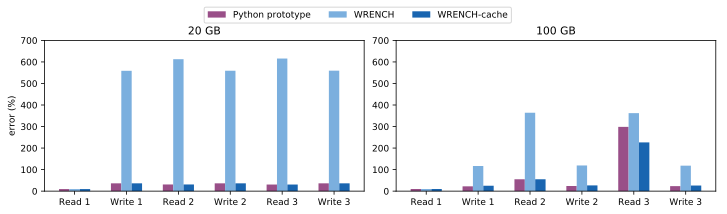
\includegraphics[width=\linewidth]{result/single/figures/single_errors.pdf}
                   \vspace*{-0.7cm}
                   \caption{Absolute relative simulation errors}
                   \vspace*{0.5cm}
                   \label{fig:single_error}
                \end{subfigure}
            \begin{subfigure}{\linewidth}
                \centering
                %    Gray shades represent task phases (read, compute and write).
                %    Lines represent memory usage along pipeline execution time.}
                   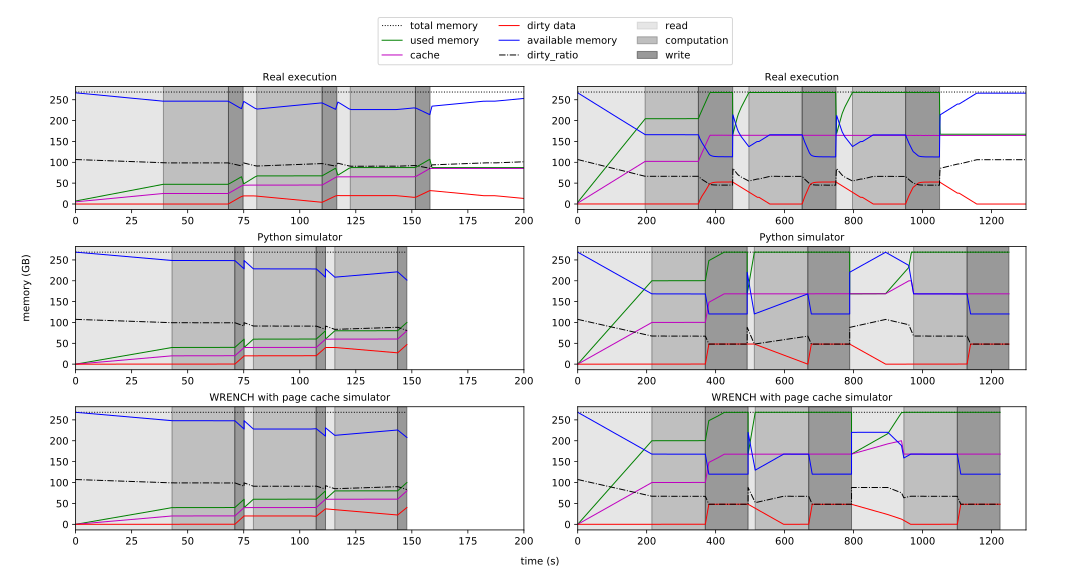
\includegraphics[width=\linewidth]{result/single/figures/single_memprof.pdf}
                   \vspace*{-0.7cm}
                   \caption{Memory profiles \tristan{Remove trailing
                   whitespace for 20GB graphs (xmax should be about 160s,
                   not 200s)} \tristan{Find a way to add Read 1, Write 1,
                   Read 2, etc on the graphs, perhaps at the top of the
                   real execution graphs}}
                   \vspace*{0.5cm}
                   \label{fig:single_memprof}
            \end{subfigure}
            \begin{subfigure}{\linewidth}
                \centering
                   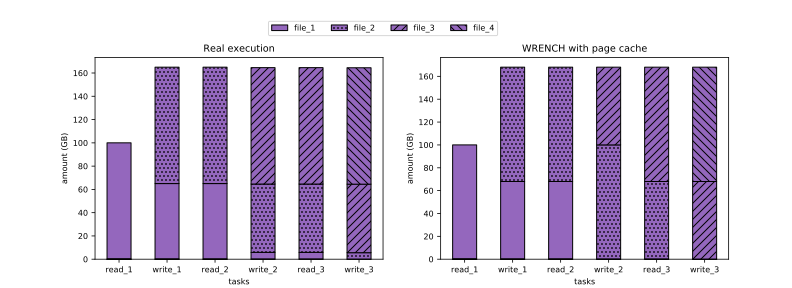
\includegraphics[width=1.05\linewidth]{result/single/figures/cached_files.pdf}
                   \caption{Cache contents \emph{after} application I/O operations}
                %    \textcolor{red}{Update real results of 20GB}}
                   \label{fig:single_cache}
            \end{subfigure}
            \caption{Single-threaded results}
            \end{figure*}



        \subsection{Concurrent application (local storage)}

            \begin{figure*}
            \begin{subfigure}{\linewidth}
                \centering
                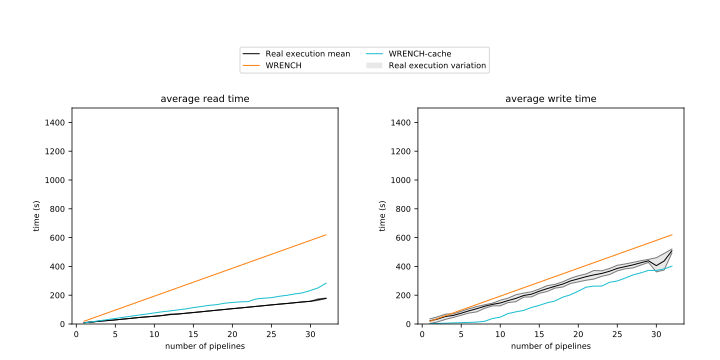
\includegraphics[width=\linewidth]{result/multi/figures/multi_local.pdf}
            \end{subfigure}
            \caption{Concurrent results with 3~GB files (averages on 5 repetitions)}
            \label{fig:multi_local}
            \end{figure*}

            The page cache model notably reduces \wrench's simulation error
            for concurrent applications executed with local I/Os
            (Figure~\ref{fig:multi_local}). For reads, \wrench-cache still
            slightly overestimates reality, due to the discrepancy between
            simulated and real read bandwidths mentioned before. For writes,
            \wrench-cache slightly underestimates reality for the same reason. The plateau
            ending around 7 concurrent applications in the \wrench-cache writes
            marks the limit beyond which the page cache is saturated with dirty data
            and needs flushing \tristan{why is there no plateau in real life?}.

        \subsection{Remote storage (NFS)}

            \begin{figure*}
            \begin{subfigure}{\linewidth}
                \centering
                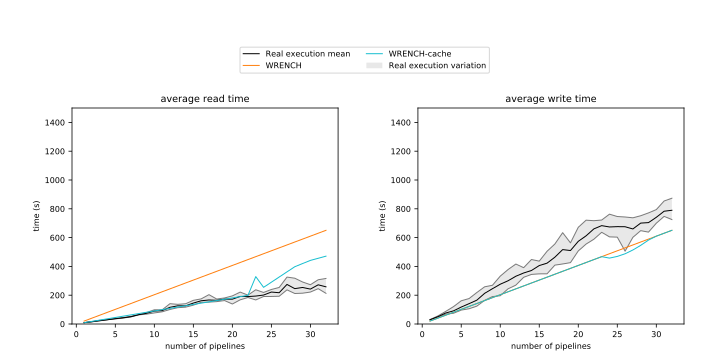
\includegraphics[width=\linewidth]{result/multi/figures/multi_nfs.pdf}
            \end{subfigure}
            \caption{NFS results with 3~GB files (averages on 5 repetitions)}
            \label{fig:multi_nfs}
            \end{figure*}

            Page cache simulation importantly reduces the simulation error
            on remote storage as well (Figure~\ref{fig:multi_nfs}). This
            manifests only for reads, as only writethrough cache was
            enabled in the NFS server. Both \wrench and \wrench-cache
            underestimate write times due to the discrepancy between
            simulated and real bandwidths mentioned previously. For reads,
            this discrepancy only impacts the results beyond 22
            applications since before this threshold, most reads result in cache
            hits.
            % \tristan{Dzung, pls check that.}.
            % Yes, disk reads appear from 23 apps indeed.

        \subsection{Real application}

        \subsection{Overhead comparison}
        As is the case for \wrench, simulation time with \wrench-cache scales
        linearly with the number of concurrent applications
        (Figure~\ref{fig:multi_time}, p \textless $10^{-24}$). However, the page
        cache model substantially increases simulation time by
        application, as can be seen by comparing regression slopes in
        Figure~\ref{fig:multi_time}. Interestingly, \wrench-cache is faster with 
        NFS I/Os than with local I/Os, most likely due to the use of writethrough
        cache in NFS, which bypasses flushing operations.
        \begin{figure}
            \begin{subfigure}{\columnwidth}
                \centering
                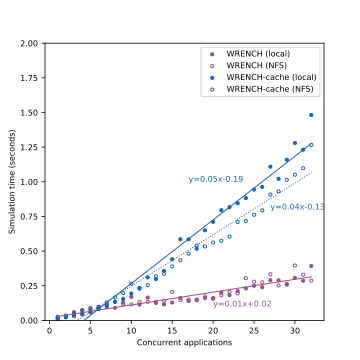
\includegraphics[width=\linewidth]{result/multi/figures/simulation_time.pdf}
            \end{subfigure}
            \caption{Simulation time comparison. \wrench-cache scales
            linearly with the number of concurrent applications, albeit
            with a higher overhead than \wrench.}
            \label{fig:multi_time}
            \end{figure}


    \section{Conclusion}
    \label{discussion}
    We designed a model of the Linux page cache and implemented it in
    the \simgrid-based \wrench library to simulate distributed
    applications. Evaluation results show that our model very
    substantially improves simulation accuracy, decreasing absolute
    relative simulation errors up to 9$\times$ (see results of
    the single-threaded experiment).
    Our page cache model is publicly available
    in the \wrench GitHub repository.

    Page cache simulation would be instrumental in a number of studies.
    For instance, it is now common for HPC clusters to run 
    application jobs in Linux control groups (cgroups), where resource consumption 
    including memory is controlled. 

    With the page cache, I/O times are strongly dependent on the amount of
    available memory, which is itself impacted by the use of anonymous
    memory by applications. A more accurate simulation of application
    memory consumption would therefore be a relevant future direction to
    further improve I/O simulation.
    
    I/Os remain much more complex than is currently available in simulation
    models.  


        Simulation results could be made even more accurate by a deeper
        investigation of page cache flushing and eviction order. 
        The availability of asymmetrical bandwidths in the
        forthcoming \simgrid release will also directly improve our
        simulation accuracy.
        
        Relevant future work includes simulating
        application memory consumption, random I/O, file readahead and
        persistent disk storage.

        \tristan{discussion could be fleshed out. cgroups}

        \section{Acknowledgments}
The computing platform used in the experiments was obtained with funding
from the Canada Foundation for Innovation.

\bibliographystyle{IEEEtran}
\bibliography{citation}

\end{document}
